\section{Fast R-CNN}

The author of R-CNN later implemented Fast R-CNN to reduce the runtime and space complexity while improving detection accuracy. Fast R-CNN is implemented in Python and C++. Like the R-CNN model, Fast R-CNN can be used along with any convolutional neural network. One very deep CNN in 2015 is VGG16, described in \cite{vgg16_2014}. Comparing the performance of Fast R-CNN with VGG16 versus R-CNN with VGG16 trained on the PASCAL VOC 2012 dataset, the author noted that Fast R-CNN is 9 times faster at train-time, 213 times faster at test-time, while achieving a higher mAP score \cite{fast_rcnn_og}. We will overview the architecture of Fast R-CNN, followed by discussing the design decision that helps Fast R-CNN achieve higher mAP.

The overall architecture of Fast R-CNN can be thought of as four steps \ref{fig:fast_rcnn_archite}. The network takes an image and a set of ROI as inputs. Comparing Fast R-CNN with R-CNN, which takes an image as an input and then generates ROIs with selective search, the type of input data between the two models is not equivalent. Thus we assume Fast R-CNN also performs the selective search algorithm at the start of the model. In the second step, Fast R-CNN generates a feature map for the entire image by running the input image through a CNN. In step three, for each proposed ROI, the model uses the ROI pooling layer to extract a feature matrix from the image feature map in step two. The ROI pooling layer is also responsible for warping the feature matrix to a pre-defined fixed-length feature vector. Each ROI feature vector is then processed by multiple fully connected layers and branched into the softmax classification output layer and bounding box regression output layer in step four. The model's learning with two output branches is possible with the use of multi-task loss.

\begin{figure}[!ht]
    \centering
    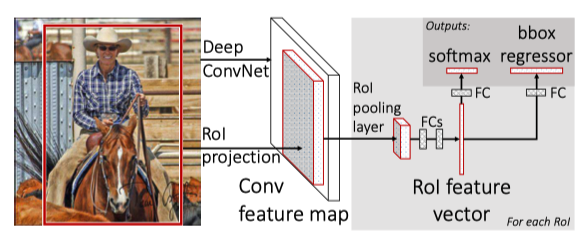
\includegraphics[width=4in]{figures/fast_rcnn_archiet.png}
    \caption{Fast R-CNN Overall Architecture \cite{fast_rcnn_og}} \label{fig:fast_rcnn_archite}
\end{figure}

Comparing the architecture of R-CNN and Fast R-CNN, there are three main differences between the two models. The first difference is that Fast R-CNN generates the feature map for the entire input image instead of each ROI individually. This means Fast R-CNN only applies CNN to image one and shares the feature maps across ROIs. Fast R-CNN behavior holds several advantages compared to treating ROIs individually, like in the R-CNN model. These advantages are reducing the use of disk storage, reducing redundancy operation performed on overlapping ROI, and sharing computation power and memory used between ROIs in the same image, thus improving the performance at test-time \cite{fast_rcnn_og}. Sharing the feature map and memory data between ROIs also allows the model to be trained faster. The author reported that training Fast R-CNN by examining multiple ROIs in an image allows the model to convert roughly 64 times faster compared to when trained with ROIs from different images. The second difference is the ROI pooling layer. Instead of wrapping pixel in a tight box like in R-CNN, Fast R-CNN achieve a similar transformation using max-pooling and names it the ROI pooling layer. The layer divides the $h \times w$ feature matrix into a pre-defined $H \times W$ grid where each subwindow in the grid has the size of $\frac{h}{H} \times \frac{w}{W}$. The ROI pooling layer then performs max-pooling on each subwindow, thus reducing the overall dimension of the ROI. The third difference is going from multi-stage training in R-CNN to single-stage multi-task training in Fast R-CNN. In R-CNN, the model must be completely trained with class-specific SVM before being trained with class-specific bounding box regressor, and these tasks also are performed in the same sequence in the test time. On the contrary, Faster R-CNN has the softmax classifier and bounding box regressor as sibling output layers. Fast R-CNN model generates a multi-task loss $L$ for each ROI and uses the loss $L$ as a metric to jointly train both the softmax classifier and bounding box regressor branches. The multi-task loss $L$ is generated from the difference between the truth label, truth box, and predicted label, predicted box perspectively. The author suggested that employing a multi-task learning scheme would improve performance, as the network's shared components must be general and precise enough to produce correct results for both classifier and bounding box regressor branches \cite{fast_rcnn_og}. The author also reports that Fast R-CNN with multi-task learning consistently achieved higher mAP scores than stage-wise training across different CNN implementations.

% \begin{figure}
%     \begin{minipage}[!ht]{6cm}
%         \woopic{rcnn_custom_draw.png}{.1}
%         \par
%         % \caption[What goes in the List of Figures]{Left}
%     \end{minipage}
    
%     \begin{minipage}[!ht]{6cm}
%         \woopic{fast_rcnn_custom_draw.png}{.1}
%         % \end{picture}
%         \par
%         % \caption{Right}
%     \end{minipage}
% \end{figure}
